\chapter{Continuous adversarial learning}\label{ch:learning}

Many people who build or buy security systems bring a belief about learning that the rest
of computing has taught them. A system that watches for attacks, records each one that
succeeds and adapts its defences grows stronger with every attempt. Spam filters work this
way, and so do the fraud models of commercial banks. Carried over to disclosure control,
the belief says that a system which keeps searching a register for weaknesses, learns which
protection settings resist the attacks it has found, and tries again whenever a candidate fails,
will in time make a release safe against hacking. The belief has a sound core. A system that
never searches finds nothing, and a system that searches without learning spends its effort
where it has already looked. The extension of November 2026 on which this part of the
book is built takes that core as its central research direction: a system that keeps searching
for disclosure weaknesses, learns from measured attack outcomes and identifies stronger
protection before a release is authorised.

The belief fails at the step that looks most like diligence, which is trying again. Take a
release whose true risk is $0.201$ against a tolerance of $0.2$, so that any certificate it receives is
false. Audit it with 500 simulated attacks and judge the audit by an exact one-sided bound
at the 5 per cent level. When an attempt fails, let the system learn what it can, draw fresh
targets and try again, judging each new attempt at 5 per cent, up to 20 attempts. Over 2,000
simulated programmes the release was certified in 50.15 per cent of them.
% source: draft 2 text, Chapter 18 opening
Had the same 5 per cent been divided among the 20 attempts before the first one ran, the share would
have been 4 per cent. Chapter~\ref{ch:monitoring} reported the same split from an older script over 20,000
programmes, 51.0 against 3.9 per cent; the extension's evidence run reproduces it with the
engine's own code.

This chapter asks one question: what may a system that keeps learning about attacks claim about a
release, and what has to stand between its learning and the decision to publish? The answer takes
four sections. Section~\ref{c18:sec-observe} fixes what the learning system observes.
Section~\ref{c18:sec-gate} separates the power to propose from the power to admit, and
Section~\ref{c18:sec-cycle} places both in a cycle. Section~\ref{c18:sec-leak} shows what repeating the
cycle does to the error, and Section~\ref{c18:sec-found} says what the system can do about a weakness in a
file that is already out.

\section{What the learning system observes}\label{c18:sec-observe}

The system learns from development cases. For case $i$, let $x_i$ describe the permitted
characteristics of the data and its release history, $\theta_i$ the protection setting proposed for it, and $a_i$ the attack scenario. A versioned attack evaluator runs the attack and returns two integers: $K_i$
successes in $B_i$ trials. A predictor with parameters $\phi$ then estimates
\begin{equation}\label{c18:eq-pred}
\widehat r_\phi(x_i,\theta_i,a_i)\approx \Prob\{\text{attack succeeds}\mid x_i,\theta_i,a_i\}.
\end{equation}
The conditioning in \eqref{c18:eq-pred} is fuller than it looks. It includes the declared law from which
targets are drawn and the convention on membership, whether success is counted over all
targets or only over those in the release. These are the objects of Chapter~2, and Chapter~19
returns to them for releases that change over time. When an attack uses several releases, $x_i$
has to describe their history, or the evaluator has to receive the whole permitted history. A
predictor trained on single releases cannot be assumed to predict pooled disclosure, for the
reason Chapter~\ref{ch:programmes} proved: no function of per-release risks bounds the pooled one.

The outcome is kept as two integers because a rate throws away the information that says
how much to trust it. A success rate of $0.1$ measured on ten trials and the same rate measured
on ten thousand carry very different weight in a binomial likelihood, and the exact bounds
of Chapter~\ref{ch:estimate} need $K$ and $B$ separately. The engine enforces this. A \texttt{MeasurementRecord}
refuses a success count or a trial count that is not an integer, and each record names the
scenario, the mechanism, the target law, the conditioning event, the data split, the stream
of random seeds, and SHA-256 digests of the data and of the evaluator. A record in the
final-audit split must also name the hash of the frozen plan it belongs to and the share of the
error budget allocated to it. Two rows that differ in any of these identifiers measure different
experiments, and the learning system may not pool them without saying so.

The same discipline applies across kinds of harm. Linkage, membership inference, attribute inference and reconstruction are separate harm classes, and Chapter~\ref{ch:credit} found five
distinct harms in one credit register. They need not share a denominator, a tolerance or a
measure of utility. A training objective that pools them has to represent each consistently
first, or the predictor will learn an average of quantities that answer different questions.

A language model can enter at this point, as Chapter~\ref{ch:proposals} described. It can suggest an
auxiliary source the library has missed, a combination of releases, or a strategy nobody has
tried. A reviewer and a deterministic evaluator then turn the suggestion into an experiment
that can be run, and the label is the count the experiment returns. What the model expected
to happen is not a label. Proposition~\ref{c14:prop-labels} showed why: only measured counts carry information about the risk. A predictor trained on counts that a model generated learns the
generator's frequency, which is the model's guess about the risk and not the risk.

Naledi's first task was an inventory of what the Bank already knew in this form. Most
of it was in tables of rates from the work of Chapter~\ref{ch:credit}, and an older helper in the software
had rebuilt counts by multiplying rates by the number of replicates. The engine now takes
counts directly and warns when it has to rebuild them. Grace, reading the inventory, asked
for one thing: that each row should say how many trials stood behind it. Naledi regenerated
the rows from the stored runs, and the committee's first exhibit became a list of integer pairs
with their identifiers.

\section{Learning proposes; evidence authorises}\label{c18:sec-gate}

The decision to release is a constrained choice. At review epoch $t$, let $\mathcal A_t$ be the family of
attacks the institution requires, $\Theta_t$ the frozen set of candidate protection settings, and $V_t(\theta)$
the usefulness of a release under setting $\theta$ for its declared analyses. For each required attack
$a$, let $U_{a,t}(\theta)$ be a valid upper confidence bound on the attack's success and $\tau_{a,t}$ its approved
tolerance. The release gate chooses
\begin{equation}\label{c18:eq-gate}
\theta_t^\ast\in\arg\max_{\theta\in\Theta_t} V_t(\theta)\quad\text{subject to}\quad U_{a,t}(\theta)\le\tau_{a,t}\ \text{for every }a\in\mathcal A_t .
\end{equation}
This is the selection problem of Chapter~\ref{ch:selection} with one change of emphasis. There the candidates
were a grid of minimum cell counts and the order of testing was fixed in advance; here
the candidates may have been proposed by a learning system, and the gate has to keep its
guarantee however they were found.

Four rules turn \eqref{c18:eq-gate} into something an institution can operate. A missing audit coordinate is not zero risk: a candidate with no bound for a required attack fails that attack. If
the feasible set is empty, the release is withheld, redesigned or moved to a more restricted
access route. The learning system never relaxes a tolerance to obtain a pass. The institution
may reconsider its tolerances, but through the governance process of Chapter~8, with a new
decision record and a named owner. And the predictor's estimate \eqref{c18:eq-pred} never enters the
constraint. The network can rank candidates, draw up a shortlist or decide where audit
effort should go, but the bound $U_{a,t}$ comes from fresh audit attacks under the declared sampling design, and when several candidates are inspected the bounds are simultaneous, as in
Proposition~\ref{c14:prop-gate}, or come from a sequential procedure with its own proof, as in Chapter~\ref{ch:monitoring}.

\begin{proposition}[The release gate]\label{c18:prop-gate}
Let $\mathcal D$ be all development information, including every model fitted and every candidate proposed. Conditional on $\mathcal D$, fix the candidates $\Theta_t$, the required attacks $\mathcal A_t$,
the tolerances and the audit design, and let $E$ be the event that $r_a(\theta)\le U_a(\theta)$ for every pair $(\theta,a)$
for which an audit bound exists. Suppose $\Prob(E\mid\mathcal D)\ge 1-\alpha$. Then:
\begin{enumerate}
\item for any utility $V_t$, the probability that the gate releases a candidate $\theta$ with $r_a(\theta)>\tau_a$ for some required $a$ is at most $\alpha$;
\item adding a required attack, or lowering a tolerance, never enlarges the feasible set;
\item if a missing coordinate were counted as zero risk, no bound on the probability in part 1 below one would hold.
\end{enumerate}
\end{proposition}

\begin{figure}[ht]
\centering
\begin{tikzpicture}
\begin{axis}[
  width=0.8\textwidth, height=6.2cm, ybar, bar width=16pt,
  ylabel={Upper bound on success}, ymin=0, ymax=0.5,
  symbolic x coords={Floor 75,Floor 150}, xtick=data, enlarge x limits=0.5,
  legend style={at={(0.03,0.97)},anchor=north west,draw=none,font=\scriptsize,fill=white}]
\addplot[black,fill=gray!45] coordinates {(Floor 75,0.104) (Floor 150,0.109)};
\addplot[black,pattern=north east lines] coordinates {(Floor 75,0) (Floor 150,0.42)};
\draw[dashed] (axis cs:Floor 75,0.12) -- (axis cs:Floor 150,0.12) node[right,font=\scriptsize]{tolerance 0.12};
\legend{External: six vintages and history, Insider: exact exposure}
\end{axis}
\end{tikzpicture}
% source: draft 2, Figure 18.1 and the text of Section 18.2
\caption{The bounds the release gate received in the extension's evidence run. Solid grey bars
are the external adversary who pools six vintages and knows the loan's history; hatched bars are the
insider. The dashed line is the tolerance. The floor of 75 has no insider audit, which the gate counts
as a failure (no hatched bar is drawn there). With the insider required, no candidate is feasible and the gate withholds; with only the
external adversary required, it releases the floor of 75.}
\label{c18:fig-gate}
\end{figure}

The proposition puts the gate's whole guarantee in the event $E$. Nothing in it depends
on how good the predictor was, how the candidates were proposed, or how the utility was
estimated. A poor predictor costs audit effort and may leave a useful candidate off the
shortlist. It cannot raise the chance that an unsafe candidate is released, because it never
touches the bounds. This is the old design principle of separation of privilege, under which
a protection mechanism should need two keys \citep{saltzer1975}: learning holds
one key, which is the power to propose, and the audit holds the other, which is the power to
admit. Part 3 is the reason the gate refuses to treat silence as safety. A candidate for which
no one has run the insider attack has not passed the insider attack.

Utility needs evidence of its own. If $V_t$ is estimated with uncertainty, the uncertainty
should be recorded and tested on the analyses the release is meant to serve. A gate can stay
statistically valid while a badly estimated utility picks a release that helps nobody. That is a
failure of a different kind from false certification, and it should be reported as such.

The extension's evidence run applies the gate to two candidates from the credit register
of Chapter~\ref{ch:credit}: a minimum cell count of 75, which keeps 45 per cent of loans, and one of
150, which keeps 20 per cent. The tolerance is $0.12$ for every attack. Figure~\ref{c18:fig-gate} shows the
bounds the gate received. For the external adversary who pools six vintages and knows the
loan's history, the bounds are $0.104$ at 75 and $0.109$ at 150, both below the tolerance. For the
insider, the gate received a bound of $0.42$ at 150, close to the $0.416$ that Chapter~\ref{ch:credit} reports for
the insider even at a floor of 300, and no bound at all at 75. When the insider is a required
attack the gate returns \textsc{withhold}: the floor of 150 fails the insider and the floor of 75 is
missing the insider coordinate. When only the external attack is required the gate returns
\textsc{release} and chooses 75, the candidate that keeps more loans.

The example also shows the limit of what the gate can check. The run files both external
bounds under one attack name, but they come from two rows of Table~13.4: $0.104$ is the
confirmed bound at 75 for the adversary who holds one reading of exposure, and $0.109$ is the
bound at 150 for the adversary who holds a reading in every vintage. The second adversary
needs a floor of 150, so had the gate been given that adversary for both candidates, 75 would
have failed it. The gate decides on the coordinates it is handed. It cannot notice that two of
them answer different questions. That check belongs to the person who writes the plan, and
to the identifiers on each measurement record, which is why the record names the
scenario as well as the attack.

\begin{figure}[ht]
\centering
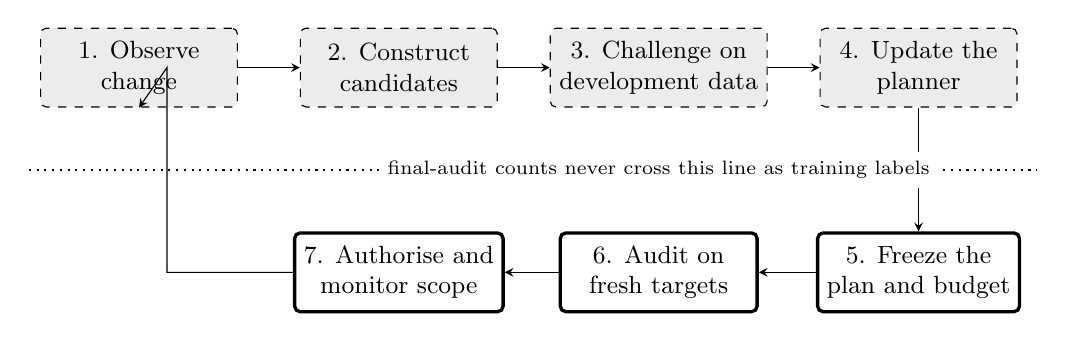
\begin{tikzpicture}[>=stealth,box/.style={draw,rounded corners=2pt,minimum width=2.5cm,minimum height=1.0cm,align=center,font=\small},
  learn/.style={box,dashed,fill=gray!15},decide/.style={box,very thick}]
\node[learn] (a) at (0,0) {1. Observe\\ change};
\node[learn] (b) at (3.3,0) {2. Construct\\ candidates};
\node[learn] (c) at (6.6,0) {3. Challenge on\\ development data};
\node[learn] (d) at (9.9,0) {4. Update the\\ planner};
\node[decide] (e) at (9.9,-2.6) {5. Freeze the\\ plan and budget};
\node[decide] (f) at (6.6,-2.6) {6. Audit on\\ fresh targets};
\node[decide] (g) at (3.3,-2.6) {7. Authorise and\\ monitor scope};
\draw[->] (a)--(b); \draw[->] (b)--(c); \draw[->] (c)--(d); \draw[->] (d)--(e);
\draw[->] (e)--(f); \draw[->] (f)--(g); \draw[->] (g.west)--++(-1.6,0)--++(0,2.6)--(a.south);
\draw[dotted,thick] (-1.4,-1.3)--(11.4,-1.3);
\node[font=\scriptsize,fill=white] at (6.6,-1.3) {final-audit counts never cross this line as training labels};
\end{tikzpicture}
\caption{The seven stages of the protection cycle. Dashed boxes on a grey ground are learning:
they may use any development evidence and change as often as needed. Heavy boxes on a white
ground are evidence and decision: their plans are frozen before outcomes exist, and their counts are
stored for governance. The dotted line marks the separation of Section~\ref{c18:sec-leak}.}
\label{c18:fig-cycle}
\end{figure}

When Naledi showed the committee the withheld decision, the chair asked the obvious
question: could the system not search until it found a setting that passed the insider? Naledi
pointed to Proposition~\ref{c13:prop-insider}. An adversary who reads exposure precisely separates candidates in a cell of any size, so no minimum cell count can stop Pieter, and rounding exposure
to one significant figure only brings his success with no floor down to $0.388$. The search
could go on for ever and the feasible set would stay empty. What the chair could decide,
and the system could not, was whether Pieter belonged in the required family for this file.
Tom\'as would work in the Bank's secure environment, with outputs checked before they left,
and no reporting lender's staff had access to it. The chair recorded the insider as outside the
scope of that access route, signed the external-only plan, and the gate chose 75 for the secure
room. The decision record says who removed the insider from $\mathcal A_t$, and why.

\section{The protection cycle}\label{c18:sec-cycle}

The gate is one stage in a cycle that the extension sets out in seven stages, drawn in
Figure~\ref{c18:fig-cycle}. The first stage observes change: new data, a shift in the distribution of the register, altered access, an additional release, a new auxiliary source outside the institution,
or a newly demonstrated attack. For each change it records whether the change could invalidate the scope of an existing certificate. The second constructs candidate releases with
explicit mechanism parameters and a declared assessment of their utility, while the confidential data stay protected throughout development. The third challenges the candidates.
It runs approved attacks on development evidence, searches across attacker capabilities and
pooled release histories, and keeps the searches that failed as well as those that succeeded.
The fourth updates the planner: it fits or recalibrates the predictor, compares it with simple baselines, inspects the subgroups where it fails, and versions the data, evaluators and
models so that any apparent improvement can be traced.

The last three stages are of a different kind, and the figure marks them differently. The
fifth freezes the proposed decision. Before any final outcome is observed, it registers the candidate settings, the required attacks, the tolerances, the target laws, the audit sample design
and the allocation of the programme's error budget. The sixth audits independently, running fresh attacks through the registered path, and approves a release only if every required
condition passes and the policy authority signs. The seventh monitors the approved scope
for the changes that would trigger another review, and keeps clear the difference between a
certificate for a specified release and an open-ended claim about the future.

The order of stages five and six carries the statistics. Chapter~\ref{ch:protocol} proved that declarations
must precede the evidence they govern (Proposition~\ref{c16:prop-order}), and the cycle applies that order
once per pass. Learning in stages one to four may be as adaptive as the analyst likes, because
Proposition~\ref{c18:prop-gate} conditions on everything that happened there. What it may not do is reach
forward into stage six.

Continuous, in this design, describes the search and not the signing. The predictor can
be refitted weekly and the search can run every night. Release authorisation remains a controlled, versioned decision, taken at the pace at which the data and the adversary's information change. A register whose exposures move monthly and whose users receive monthly
files needs a monthly review; a public table published once a year does not.

Naledi ran the first pass for Tom\'as's second file. Stage one found the largest change: the
new file would add six months to a history Tom\'as already held, so the pooled adversary
would see twelve vintages where the certificate had assumed six. That change took the
request outside the old scope, and Chapter~19 shows why a longer history of a changing
register cannot be assessed by reading the old certificate forward. Stage three searched,
stage four refitted the planner on the development counts, and on Thursday Naledi froze a
plan with three candidate floors and the external attack only, as the chair had recorded.

\begin{remark}[Check the retry study yourself]
The two figures at the head of the chapter come from a short simulation, and the reader can rerun it. A release has true risk $0.201$ and the tolerance is $0.2$, so any certificate is false. Each attempt draws 500 attacks and certifies when the exact one-sided upper bound at level $\alpha$ is at most $0.2$. Twenty attempts at $\alpha=0.05$ certified the release in $0.501$ of 4,000 simulated programmes; the same twenty attempts at $\alpha=0.05/20$ did so in $0.041$ of them. The Bayesian betting audit of Example~\ref{c18:ex-bet} can be replayed in a few lines in the same way: with the stated forecast the wealth after the first four attacks is $1.023$, $1.057$, $1.101$ and $0.705$ and the audit certifies at attack 55, and a clean run reaches $4.0$ at attack 20 and $22.2$ at attack 37. A fixed audit that certifies only on zero successes needs $\lceil\ln 0.05/\ln 0.88\rceil=24$ attacks. These were recomputed from the formulas, not copied from the extension's run, and they agree with it.
\end{remark}

\section{Leakage across successive cycles}\label{c18:sec-leak}

A cycle that runs once has a clean separation between development and audit. A cycle that
runs every month does not, unless the institution builds one. The danger is that the final
audit of one pass becomes training data for the next, and that the next pass then certifies
a candidate on the same favourable sample that taught the planner to propose it. Reusing
an audit sample after retraining is not independent verification. It is the scan of Chapter~5,
in which the same counts that pick the winner are asked to certify it, and Proposition~\ref{c05:prop-scan}
measured the cost of that. Machine learning met the same problem in the holdout set that
is consulted again after every round of model changes, and found that reuse invalidates it
unless access is rationed \citep{dwork2015}.

The conservative rule, and the one the engine implements, is that final-audit outcomes
are stored for governance and never used as development labels. The function that loads
training rows refuses a request that includes the final-audit split, so a permissive query
cannot leak final outcomes into development by accident. A failure found in an audit is
not lost. It triggers a separately registered development investigation, which draws its own
fresh measurements.

A more permissive design is possible, and the next proposition says what it would need.
Think of the programme as a sequence of cycles, and let $\mathcal F_{\ell-1}$ hold everything known before
the final audit of cycle $\ell$ begins, including the final audits of every earlier cycle.

\begin{proposition}[Error accounting across cycles]\label{c18:prop-cycles}
Let a programme run cycles $\ell=1,2,\dots$, and let $A_\ell$ be the event that cycle $\ell$ certifies a candidate whose risk exceeds its tolerance for some
required attack. Suppose that the error allocation $\alpha_\ell$ of cycle $\ell$ is fixed by $\mathcal F_{\ell-1}$, that $\sum_\ell\alpha_\ell\le\alpha_{\rm prog}$ in
every outcome, and that $\Prob(A_\ell\mid\mathcal F_{\ell-1})\le\alpha_\ell$. Then the probability that any cycle in the programme
certifies falsely is at most $\alpha_{\rm prog}$. If instead each cycle is run at a fixed level $\alpha$ with no budget, the only
general bound after $n$ cycles is $\min(1,n\alpha)$.
\end{proposition}

The proposition lets earlier audits influence later development, and it is exact about the
price. Each cycle's audit must be valid conditional on everything before it, which in practice
means fresh targets that the earlier cycles have not touched, and each cycle's allocation must
be written down before its audit starts. The retry study at the head of this chapter is the
second part of the proposition at work: twenty attempts at 5 per cent each allow a bound of
one, and the simulation found $0.50$. Dividing the 5 per cent among the attempts restores the
first part, and the simulation found $0.04$. The conservative rule is a special case that is easier
to check, because a final audit that never reaches development cannot make a later audit's
targets depend on it.

Random seeds alone do not make two audits independent. The targets themselves can
be shared. Two releases can overlap in ways the seed does not see. And a development path
and an audit path can read the same records through different routes. Where the target is
a borrower with several loans, the dependence has to be reflected in the unit of audit. On
the register of Chapter~\ref{ch:credit} the attack recovered the exact lending relationship for $0.0855$ of
released rows and the right borrower for $0.1095$, because a borrower with several lenders can
be found through any of them. When the borrower is the person at risk, the audit samples
borrowers.

The engine's registry makes the accounting hard to forget. A programme opens with a
total error budget. A plan is registered by its hash before any outcome exists. Each attempt
reserves its share of the budget in a database transaction before the audit draws a single
target, and an attempt that fails or is abandoned keeps its spend. Two writers cannot both
spend the last of a budget, because the reservation takes the database's write lock before
it reads the amount already spent. Weaker isolation would let two transactions each read
the same balance and each write a spend, an anomaly that \citet{berenson1995} catalogue
for the isolation levels of SQL. Each attempt receives its own audit random stream, from
a seed drawn at random when the budget is reserved and recorded with the attempt, so
that it can be replayed afterwards but not computed in advance from the plan, and it stays
apart from the development streams. The registry detects a later edit to a stored plan by
recomputing its hash. It does not prove who wrote a row or when; for that an external
timestamp or an independently administered signed store is needed, and both remain open.
Dividing a fixed error among looks taken over time is an old device of clinical trials, where
an alpha-spending function fixes how much of the error each interim analysis may use \citep{lan1983}, and \citet{foster2008} let a testing programme earn back budget
from its discoveries. The registry uses the plainest version: shares fixed in advance, each
paid before its audit runs.

\begin{example}[Four reservations against one budget]\label{c18:ex-budget}
Take the programme for Tom\'as's second file with a total budget of $0.05$, and let each attempt reserve $0.0125$, a quarter of it. The
figures are illustrative. Naledi registers a plan for the floor of 50 and reserves the first share;
the registry records the attempt and reports $0.0375$ left. That audit fails and is closed as a
failure. A second reservation against the same plan leaves $0.025$, and it fails too. A plan for
the floor of 75 is registered, its reservation leaves $0.0125$, and it passes. A fourth reservation, opened by mistake, leaves nothing and is closed as abandoned. Every attempt spent
its share, so the ledger shows $0.05$ spent. A fifth reservation of $0.0125$ is refused, and so is
one of $0.001$: the programme has no budget left, and only a new decision by the committee
can open another programme. By Proposition~\ref{c18:prop-cycles}, the chance that any of the four certified
a release whose risk exceeds the tolerance is at most $0.05$. Had each attempt been judged at
$0.05$ with no ledger, the only general bound would be $4\times0.05=0.2$.
\end{example}

Sequential audits fit the same accounting. The betting audit of Chapter~\ref{ch:monitoring} fixes each bet
from the outcomes before it and stops when its wealth reaches $1/\alpha$, and Ville's inequality
bounds the chance of a false certificate by $\alpha$ \citep{ville1939,howard2021}. Testing by betting has become a general method of statistics \citep{shafer2021,ramdas2023,grunwald2024}, and betting strategies of this kind also give confidence bounds for bounded
means \citep{waudbysmith2024}. In the extension's evidence run, at a tolerance of
$0.12$ and $\alpha=0.05$, a release whose true risk sat exactly at the tolerance was certified in 46 of
1,000 runs, a rate of $0.046$ with an exact upper bound of $0.058$. Below the tolerance the audit
stopped early: the median run used 56 attacks at a true risk of $0.03$, 144 at $0.06$ and 669 at
$0.09$, and at $0.09$ it certified in 85 per cent of runs within its 1,500 attacks. A fixed audit that
certifies only on zero successes would need 24 attacks at the same tolerance. The bets came
from a Bayesian forecast, and the forecast set the cost. It did not set the error, which stayed
within its bound.

\begin{example}[The first attacks of a betting audit]\label{c18:ex-bet}
Take the evidence run's settings: tolerance
$0.12$, $\alpha=0.05$, so the audit certifies when its wealth reaches 20, and bets from a Beta$(1,9)$
forecast. Before the first attack the forecast's mean is $1/10=0.1$, so the first bet is $0.1$. If the
attack fails, the wealth is multiplied by $(1-0.1)/(1-0.12)=1.023$. The forecast moves to
$1/11=0.091$, the second failure multiplies the wealth by $0.909/0.88$, and the wealth is $1.057$;
a third failure, at a bet of $1/12$, brings it to $1.101$. Suppose the fourth attack succeeds. The
bet was $1/13=0.077$, so the wealth is multiplied by $0.077/0.12=0.641$ and falls to $0.705$.
The forecast after a success rises to $2/14=0.143$, above the tolerance, so the engine clips the
next bet to $0.12-0.012=0.108$, and each failure then adds only 1.4 per cent. The bets fall
again as failures accumulate, and the audit certifies at attack 55. Had the fourth attack failed,
the wealth would have reached $4.0$ after 20 attacks and $22.2$ after 37, and the audit would
have certified there. The fixed audit that certifies only on zero successes would stop at 24
attacks with no success and would fail outright at the fourth. The betting audit is slower
on a clean run and survives a success; it never certifies a release at the tolerance more often
than one time in twenty.
\end{example}

Grace read the registry for Tom\'as's second file a week after the decision. She found the
four attempts of Example~\ref{c18:ex-budget}, each with its share spent, and the verification of plan hashes
returned an empty list. Her question was why a failed attempt should cost anything, since
it had certified nothing. Naledi answered with the retry study: the cost of a failure is that it
buys the right to try again, and the budget is what keeps the twentieth try from being a coin
toss.

\section{After a weakness is found}\label{c18:sec-found}

A system that keeps searching will sometimes find a weakness in a release that is already
out. What it can do then depends on where the release sits. For a proposed release, the
institution can withhold it, raise the protection, reduce the detail or change the access route
before publication. For a controlled service, such as a query server or a secure environment,
an authorised response can suspend new queries, restrict access or change future outputs.
These are prospective controls. They act on what has not yet been disclosed.

A public file already copied by others cannot be made private again. Retraining the
predictor does not recall it, deleting the source copy does not recall it, and publishing a safer
replacement adds a second file to the first. The documented cases show the pattern. The film-rating data that \citet{narayanan2008} linked to public reviews had been released
for a prize contest before the linkage was published. The US Census Bureau's reconstruction
experiments on the published tables of the 2010 census led it to adopt a formal privacy
guarantee for 2020 \citep{garfinkel2019,abowd2022}; the 2010 tables remained
published, and the response protected the next census. In neither case did a later decision
lower the risk of the earlier file.

\begin{proposition}[What a later decision cannot lower]\label{c18:prop-floor}
Let release $Y_1$ be public and let $R^\ast(Y_1;B)$
be the success of the best attack, within a declared family, that uses $Y_1$ and auxiliary information $B$.
For any later releases $Y_2,\dots,Y_m$, chosen by any rule, the success of the best attack in the same family
on the whole programme is at least $R^\ast(Y_1;B)$, with equality when nothing further is released. If the
auxiliary information grows from $B$ to $B'\supseteq B$, then $R^\ast(Y_1;B')\ge R^\ast(Y_1;B)$.
\end{proposition}

The proposition is elementary, and that is its use in a committee room. It says that the
risk of a published file is a floor under every future programme that includes it, and that the
floor can rise when someone outside the institution publishes a new source, but never fall
because of anything the institution does next. A correct response to a discovered weakness
therefore documents the affected releases, reviews future publication with the earlier files
counted in the pooled attack, as Chapter~\ref{ch:programmes} requires, and follows the institution's incident
process where one applies. It must not claim that a model update erased earlier exposure.

Three months into Tom\'as's study, stage one of the cycle found a new source: a commercial data vendor had begun publishing loan sizes for listed firms. The secure room was not
affected, because nothing had left it except checked outputs. The Bank's public monthly
series was another matter. It had been published for years, and the vendor's data could
now be laid beside it. Naledi's note to the chair said what the Bank could not do, which
was recall the series, and what it could do: assess the next month's release jointly with the
published back series and the vendor's data, and coarsen it if the pooled attack failed.

\section{The claim that has to be tested}

The extension proposes a contribution with a precise name: continuous adversarial learning
for disclosure control, with independently verified release decisions. Its test is comparative. Model-assisted search and planning should either find relevant weaknesses earlier, or
keep more utility at a fixed risk criterion and a fixed compute budget, and in either case
the audit's error control must hold. The measures that would show it are attack coverage,
independently confirmed success rates, performance on the worst subgroup, release utility,
evaluator cost, reviewer effort and the rate of false certification, all under a design declared
before the experiment runs. The design has to include attacks outside the training library
and later periods of data, because a system that learns can always look good on the attacks
it was trained against.

The evidence so far is evidence about components. Of the extension's seventeen engineering steps, ten are done in the engine with tests, and one, the model of changing exposure, is half done. Three are open because they need a governed register or the joined
end-to-end experiment, and three are not built: two wait until simpler models have been
shown to fall short, and the third is a live model adapter that the Bank has chosen not to
connect. Where the book has measured the learning parts directly, the results are mixed or
negative. A small language model given the same budget covered $6.05$ scenario cells against
$13.65$ for a Sobol search, on the states where it produced a valid answer (Chapter~\ref{ch:proposals}), and
Chapter~\ref{ch:planner} examines what a deeper planner adds over a logistic one on the same counts.
The claim that the whole pipeline improves institutional release decisions is therefore unestablished. It needs steps 10, 16 and 17: authorised data in place of synthetic observations,
a joined synthetic release experiment, and validation on a governed register. Grace recorded
those three steps as conditions on any operational claim, and the committee minuted them
beside the decision for Tom\'as.

\section{The answer}

The chapter asked what a system that keeps learning about attacks may claim about a
release, and what has to stand between its learning and the decision to publish. It may claim
that it searched, what it searched, and what it found, with every finding stored as an integer
count that names its experiment. It may not claim that a release is safe against hacking, because that names no event anyone can bound, and it may not let its own predictions decide.
Between learning and publication stand three things. A gate admits only candidates whose
fresh audit bounds meet every required tolerance, fails any candidate with a missing coordinate, and withholds when nothing passes. A frozen plan and an error budget, spent before
outcomes exist, stop retries and successive cycles from buying a pass. And a person with
authority decides the required attacks, the tolerances and the access route, and signs. Under
those conditions the gate's chance of a false release is the $\alpha$ written on the plan, whatever
the learning did. A file already published stays published, and the most the system can do
after finding a weakness in it is protect the next one.

\begin{inpractice}[In practice: running a learning system beside the release gate]
Keep every development and audit outcome as an integer count of successes and trials, with
the scenario, mechanism, target law, conditioning event, split and evaluator version beside it.
Before any final audit, freeze the candidates, the required attacks, the tolerances, the target law,
the audit design and the error allocation, and record the plan's hash. Treat a missing audit coordinate as a failure. When no candidate passes, withhold, redesign or move to a more restricted
access route, and send any change of tolerance or of required attacks to the committee as a new
decision with a named owner. Spend error budget for every attempt, including those that fail or
are abandoned. Never train on final-audit outcomes. When a weakness is found in a published
file, document the affected releases and assess the next release jointly with what is already out.

\medskip\noindent\textit{In the software.} The gate is \texttt{privacy\_risk.gate.decide\_release}, which takes candidate utilities, required
tolerances and a list of \texttt{gate.Coordinate} bounds whose source must be \texttt{"audit"}. Measurement rows are \texttt{evidence.MeasurementRecord}, and
\texttt{evidence.training\_rows} refuses the final-audit split. The programme budget and frozen plans
live in \texttt{registry.Registry}, a SQLite store that reserves each share inside a write transaction. The betting audit is \texttt{betting.run\_audit}, with
bets from \texttt{betting.predictable\_bets}. The tests are in \texttt{tests/test\_ext\_learning.py}, and they replay the checks of Algorithm~18.1, Example~\ref{c18:ex-budget} and Example~\ref{c18:ex-bet}.
\end{inpractice}

\begin{mdframed}[linecolor=gray!60,backgroundcolor=gray!5]
\textbf{Algorithm \thechapter.1.} The release gate.\par\smallskip
\textit{Input.} The frozen candidates $\theta\in\Theta_t$, each with a utility $V_t(\theta)$; the required attacks $a\in\mathcal A_t$, each
with a tolerance $\tau_a$; and a list of upper bounds $U_a(\theta)$, each naming its candidate, its attack and
its source.\par
\textit{Output.} \textsc{release} with the chosen candidate, or \textsc{withhold} with none; and, for each candidate, the attacks it failed and the attacks for which it has no bound.
\begin{enumerate}
\item Refuse the inputs if there is no candidate or no required attack, if a tolerance lies outside
$(0,1]$, if a bound lies outside $[0,1]$, if a bound comes from any source other than an independent audit (a planner's prediction is refused), or if a bound names a candidate that was not frozen.
\item For each candidate $\theta$ and each required attack $a$: if no bound $U_a(\theta)$ was given, record $a$ as
missing for $\theta$; if $U_a(\theta)>\tau_a$, record $a$ as failed for $\theta$. A bound equal to the tolerance passes.
\item Call $\theta$ feasible when it has no failed and no missing attack, so that it meets every constraint
of \eqref{c18:eq-gate} with evidence (Proposition~\ref{c18:prop-gate}, part 3).
\item If no candidate is feasible, return \textsc{withhold}, name redesign and the more restricted access routes as next steps, and leave every tolerance as it was.
\item Otherwise return \textsc{release} with the feasible candidate of largest utility.
\end{enumerate}
\textit{Checks, each run against the software by the test suite:}
\begin{itemize}
\item Floors of 75 and 150 with utilities $0.45$ and $0.20$, the bounds of Figure~\ref{c18:fig-gate}, and only the external pooled attack required at $0.12$: \textsc{release}.
\item The same, the floor chosen: 75.
\item The same with the insider also required: \textsc{withhold}.
\item The same, the attack missing at the floor of 75: insider.
\item The same, the attack failed at the floor of 150: insider.
\item Only the external attack required, with the bound at 75 exactly equal to the tolerance, the floor chosen: 75.
\item A bound whose source is a planner's prediction: refused.
\item No required attack: refused.
\end{itemize}
\end{mdframed}

\section{Proofs}

\begin{proof}[Proof of Proposition~\ref{c18:prop-gate}]
Write $C$ for the set of pairs $(\theta,a)$ with $\theta\in\Theta_t$, $a\in\mathcal A_t$ and an audit
bound $U_a(\theta)$. The gate's feasible set is
\[F(\mathcal A_t,\tau)=\{\theta\in\Theta_t:(\theta,a)\in C\text{ and }U_a(\theta)\le\tau_a\text{ for every }a\in\mathcal A_t\}.\]
For part 1, let $W$ be the event that the gate releases some $\theta^\ast$ with $r_a(\theta^\ast)>\tau_a$ for some
$a\in\mathcal A_t$. If the gate releases $\theta^\ast$, then $\theta^\ast\in F$, so for every required $a$ the pair $(\theta^\ast,a)$
is in $C$ and $U_a(\theta^\ast)\le\tau_a$. On $E$ we then have $r_a(\theta^\ast)\le U_a(\theta^\ast)\le\tau_a$ for every required $a$, so $W$ does
not occur. Hence $W\subseteq E^c$ and $\Prob(W\mid\mathcal D)\le\Prob(E^c\mid\mathcal D)\le\alpha$. Taking expectations over $\mathcal D$
gives the unconditional bound. The argument used no property of $V_t$ beyond the fact that
$\theta^\ast$ is chosen from $F$, and $E$ covers every pair at once, so the choice of $\theta^\ast$ may depend on the bounds.

For part 2, if $\mathcal A_t\subseteq\mathcal A_t'$, every condition defining $F(\mathcal A_t,\tau)$ appears among those defining
$F(\mathcal A_t',\tau)$, so $F(\mathcal A_t',\tau)\subseteq F(\mathcal A_t,\tau)$. If $\tau_a'\le\tau_a$ for every $a$, then $U_a(\theta)\le\tau_a'$ implies $U_a(\theta)\le\tau_a$,
so $F(\mathcal A_t,\tau')\subseteq F(\mathcal A_t,\tau)$.

For part 3, take one candidate $\theta$, one required attack $a$ with $r_a(\theta)=1$ and no audit bound,
and any tolerance $\tau_a<1$. The event $E$ holds with probability one, since it constrains no pair.
If the missing coordinate is counted as $U_a(\theta)=0\le\tau_a$, the gate releases $\theta$ with probability
one, and $r_a(\theta)>\tau_a$. So the probability in part 1 equals one while the premise holds for every
$\alpha\in(0,1)$, and no bound below one is possible.
\end{proof}

\begin{proof}[Proof of Proposition~\ref{c18:prop-cycles}]
Cycles that are never run have $A_\ell$ empty and may be given $\alpha_\ell=0$.
By countable subadditivity, $\Prob(\bigcup_\ell A_\ell)\le\sum_\ell\Prob(A_\ell)$. For each $\ell$, the tower property and the
hypothesis give $\Prob(A_\ell)=\E[\Prob(A_\ell\mid\mathcal F_{\ell-1})]\le\E[\alpha_\ell]$. Since each $\alpha_\ell$ is nonnegative, monotone
convergence lets the sum pass inside the expectation, and
\[\Prob\Big(\bigcup_\ell A_\ell\Big)\le\sum_\ell\E[\alpha_\ell]=\E\Big[\sum_\ell\alpha_\ell\Big]\le\alpha_{\rm prog}.\]
For the second statement, if every cycle runs at level $\alpha$, the same argument with $\alpha_\ell=\alpha$
for $\ell\le n$ gives $\Prob(\bigcup_{\ell\le n}A_\ell)\le n\alpha$, and a probability is at most one. That no better general
bound exists follows from part 1 of Proposition~\ref{c06:prop-retry}: with independent attempts that each
certify falsely with probability $f$, the chance of some false certificate is $1-(1-f)^n$, which
for $f=\alpha$ and small $n\alpha$ is close to $n\alpha$ and tends to one as $n$ grows.
\end{proof}

\begin{proof}[Proof of Proposition~\ref{c18:prop-floor}]
Let $\delta$ be any attack in the declared family that uses $Y_1$ and $B$. An
adversary who holds $Y_1,\dots,Y_m$ and $B$ can run $\delta$ and ignore $Y_2,\dots,Y_m$; this attack uses the
programme and has the same success as $\delta$, whatever rule chose the later releases. The best
attack on the programme therefore succeeds at least as often as $\delta$, and taking the supremum
over $\delta$ gives the first inequality. When nothing further is released the programme is $Y_1$ alone
and the two quantities coincide. For the second statement, an attack that uses $B$ is also an
attack available to an adversary who holds $B'\supseteq B$, who can discard the extra information;
the supremum over the larger set of attacks is at least the supremum over the smaller.
\end{proof}
